%- HandOut Flag -----------------------------------------------------------------------------------------
\makeatletter
\@ifundefined{ifHandout}{%
  \expandafter\newif\csname ifHandout\endcsname
}{}
\makeatother

%- D0cum3nt ----------------------------------------------------------------------------------------------
\documentclass[beamer,10pt]{standalone}   
%\documentclass[beamer,10pt,handout]{standalone}  \Handouttrue  

\ifHandout
	\setbeameroption{show notes} %print notes   
\fi

	
%- Packages ----------------------------------------------------------------------------------------------
\usepackage{custom-style}
\usetikzlibrary{positioning}
\usepackage{multicol}


%--Beamer Style-----------------------------------------------------------------------------------------------
\usetheme{toninus}
\usepackage{animate}
\usetikzlibrary{positioning, arrows}
\usetikzlibrary{shapes,shapes.callouts}

\begin{document}

%-------------------------------------------------------------------------------------------------------------------------------------------------
\begin{frame}{Observables}
	An observables is:
	\vfill
	\begin{columns}[T]
		\begin{column}{0.5\textwidth}
			\begin{itemize}
				\item a procedure to read a certain quantity (a number) out of any state of the system
				\item<2-> a quantity that can be measured with a device. 
			\end{itemize}				
			%
			\vspace{.5em}
			\onslide<3->{
				\begin{exblock}[Pendulum inclination]
					Measure the inclination of the rod with a goniometer.
				\end{exblock}			
			}
			%
			\vspace{.5em}
			\onslide<4->{
				\begin{mathblock}
					Observables are given by smooth functions on the phase space $M$:
					\begin{displaymath}
						\mathcal{O}=C^{\infty}(M)~.
					\end{displaymath}
				\end{mathblock}
			}
		\end{column}
		\begin{column}{0.5\textwidth}
			\begin{center}
				\includegraphics<1>[width=.9\textwidth]{Pictures/pendo60-nogonio}
				\includegraphics<2>[width=.9\textwidth]{Pictures/pendo60}
				\includegraphics<3>[width=.9\textwidth]{Pictures/observo}
				\only<3>{
					\tikz[overlay,remember picture]
					{
						\node[ellipse callout,fill=white!50,
			               draw=black,
			               anchor=base]            
			            	 (base) at ($(current page.east)+(-5,3)$) [rotate=-0,text width=1.5cm,align=center,callout relative pointer={(-.3,-.8)}] 
			            	 {Measure: \\$\theta=\pi/3$\\$\phantom{\theta}\cong 1.05$};
					}	
				}
				\only<4>{
					\resizebox{.9\textwidth}{!}{				
						\begin{tikzpicture}
							\pgfmathtruncatemacro\steps{4}
							\pgfmathtruncatemacro\mintheta{-120}
							\pgfmathtruncatemacro\maxtheta{-60}
							\pgfmathsetmacro\deltatheta{(\maxtheta-\mintheta)/(\steps)}
							\pgfmathsetmacro\viewpitch{30}
							\pgfmathsetmacro\diam{2}
							\pgfmathsetmacro\H{4}
							\pgfmathsetmacro\deltaH{(\H)/(\steps)}
							\pgfmathsetmacro\X{\diam}
							\pgfmathsetmacro\Y{\diam*sin(\viewpitch)}	
							\pgfmathsetmacro\vel{\diam/4}	
		
							\draw[green,dashed,fill=green!20] (0,0) ellipse ({\X} and {\Y});
							%\draw [blue,dashed] (-1.25,-3.5) arc (180:360:1.25 and -0.5);
							\draw[green,dashed,fill=green!20] (0,-{\H}) ellipse ({\X} and {\Y});
							\draw [blue,dashed] (-{\X},-{.5*\H}) arc (180:360:{\X} and -{\Y});
							\draw [green](-{\X},0) -- (-{\X},-{\H});
							\draw [green]({\X},-{\H}) -- ({\X},0);  
							\fill [green!80,opacity=0.5] (-{\X},0) -- (-{\X},-{\H}) arc (180:360:{\X} and {\Y}) -- ({\X},0) arc (0:180:{\X} and -{\Y});
							\draw [blue](-\X,-{.5*\H}) arc (180:360:{\X} and {\Y});

							\foreach \i in {0,1,...,\steps}{
								\pgfmathsetmacro\h{-\i*\deltaH}
								\pgfmathsetmacro\theta{\mintheta + \i*\deltatheta}	
								\pgfmathsetmacro\thetalabel{-\theta -90}	
									
								\draw[red,-stealth] (0,\h)++({cos(\theta)*\X},{sin(\theta)*\Y}) node[draw,cross out]{}  -- (5,{pi*2*(\thetalabel)/180-\H/2})node[right] {${\thetalabel}^\circ$};
							}
							\draw[->] (5,-{\H})--(5,0) node[above] {${\Theta}$}; % ordinate
						\end{tikzpicture}	
					}
				}
			\end{center}
		\end{column}
	\end{columns}
\end{frame}
\note[itemize]{
	\item Observation /Measure, procedure to extract a number from a physical system.	E.g. a measure with a device	

}
%-------------------------------------------------------------------------------------------------------------------------------------------------

%-------------------------------------------------------------------------------------------------------------------------------------------------
\begin{frame}[t]{Hamiltonian: Energy observable}
	A certain observable takes a central role:
	\vfill
	\begin{columns}[T]
		\begin{column}{0.5\textwidth}
			\begin{defblock}[Hamiltonian observable]
				Observable measuring the total energy of the system.
				\begin{displaymath}
					H = \text{Kinetic} + \text{Potential}
				\end{displaymath}
			\end{defblock}		
			\vspace{1em}
			\onslide<2->{
				\begin{exblock}[Pendulum]
					In practical terms: $H$ is a device measuring the battery charge dissipated by a motor to lift the bob to a certain height.	
				\end{exblock}
			}			
			%
		\end{column}
		\begin{column}{0.5\textwidth}
			\begin{center}
				\onslide<2->{	
					\animategraphics[autoplay,palindrome,width=\textwidth]{1}{Pictures/pendolabenergy-}{0}{1}
				}			
			\end{center}
		\end{column}
	\end{columns}
	\vfill
	\onslide<3->{
		\begin{upshotblocksimp}
			Upshot: $H$	embodies how the ambient acts on the system and the system's inertia to respond to the external forces.
		\end{upshotblocksimp}		
	}


\end{frame}
\note[itemize]{
	\item among all possible observables "Energy" has a pivotal role:
	\item Without being too philosophica. Consider our pendulum system.
	\item \emph{potential energy} account the interaction of the "ambient" with the "body".
	\item \emph{kinetic energy} is the energy of the motion.
}
%-------------------------------------------------------------------------------------------------------------------------------------------------

%-------------------------------------------------------------------------------------------------------------------------------------------------
\begin{frame}{Symplectic structure}
	\center
	\alert{Phase spaces has a canonical \underline{symplectic structure}}
	\vfill
	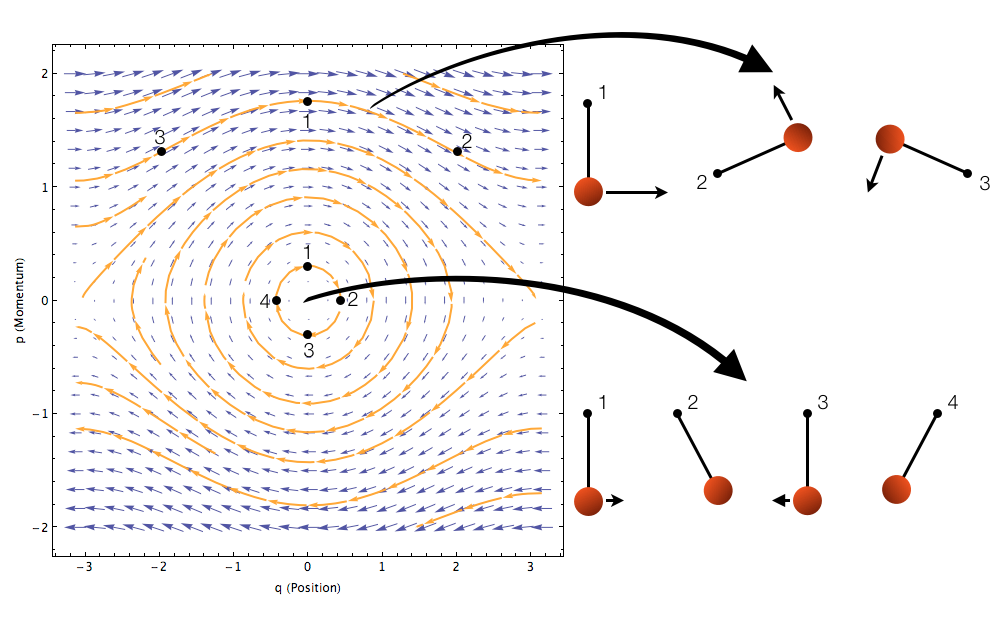
\includegraphics[width=.85\textwidth]{Pictures/pendo-hamiltonianfield}	
	\vfill
	\begin{itemize}
		\item Is  a prescription of an \emph{Hamiltonian field} $v_f$ to any observable $f$.
		\item The flow gives the evolution of the system when taking $f$ as the Hamiltonian.
		\item The Hamiltonian generates the \emph{time evolution}.
	\end{itemize}


\end{frame}
\note[itemize]{
	\item canonical i.e independent from arbitrary choices.
	\item the symplectic structure prescribes a tangent vector field to any observable quantity
}
%-------------------------------------------------------------------------------------------------------------------------------------------------

\end{document}